% KSlit.tex
% $Author$ $Date$

% \section{\KS: literature survey}
% \label{sec:KSlit}
% Vaggelis               jan 20 2007


\PC{moved here from rpo\_ks/}
%
The {1\dmn} \KSe\
as given in \refrefs{ku,siv} is (up to overall scaling factors):
\beq
    y_t=-y_x^2/2-y_{xxxx}-y_{xx}
\,,\qquad       x \in [0,L]
\,,
    \label{eq:KSeOR}
\eeq
with periodic boundary conditions in the $[0,L]$ interval. The form \refeq{ks} used
here
\beq
    u_t=uu_x-u_{xxxx}-u_{xx}
\,.
    \label{eq:KSeAP}
\eeq
is related to
\refeq{eq:KSeOR} by setting \PCedit{$u=-y_x$}.
In study of {1\dmn} \KS\ \eqva\ $x$ is interpreted as ``time",
so $y$ is a height of a front, and $y_x$ it's ``velocity".
In the literature  both forms of the equation are
referred to as the \KSe.
According to \refref{TsveTri89} the solutions of the two equations
differ considerably despite the simple way they are related.
\PC{Whatever that means? They are related by a derivative one way,
integration constant the other. Enter TsveTri89 into siminos.bib}

\subsection{\Eqva\ according to Greene and Kim}

The form of \KSe\ studied by Greene and Kim\rf{ksgreene88} is
\beq
    y_t=-4y_{xxxx}-\alpha\left(y_{xx}+\frac{1}{2}y_x^2
            -\frac{1}{4\pi}\int_0^{2\pi}y_x^2\ dx\right)
\,,\qquad       x \in [0,2\pi]
\,,
    \label{eq:KSeGreeneKim}
\eeq
with  periodic boundary condition on the interval $[0,2\pi]$.
Mean elastic energy density of a spatial profile $y(x,t)$ is defined by
\beq
    E=\frac{1}{2\pi}\int_0^{2\pi}y_x^2\, dx\,.
    \label{KSenergy}
\eeq
% \ES{This definition does not only apply to equilibria. Greene and
% Kim also study the transfer of energy between modes
% in non-stationary trajectories.}.
Taking the derivative of \refeq{eq:KSeGreeneKim}
with respect to $x$ and substituting $y_x=-u$ leads to
\[
    u_t=4u_{xxxx}+\alpha\left(u_{xx}-uu_x\right)
\,.
\]
Rescaling
\beq
    \tilde{x}=\frac{\sqrt{\alpha}}{2} x
\,,\qquad
    \tilde{t}=\frac{\alpha^2}{4} t
\,,\qquad
    \tilde{u}=\frac{2}{\sqrt{\alpha}} u
    \label{eq:GKscale}
\eeq
brings the Greene-Kim equation to the form \refeq{eq:KSeAP} used here.
The dimensionless system size $\tildeL=L/2\pi$ is related to
the Greene-Kim parameter
through $\tildeL=\sqrt{\alpha}/2$.
The system size $L=22$ studied here corresponds to $\alpha=49.0395$.

The ``kinetic energy'' reads in our units:
\PC{shouldn't there be a prefactor $\frac{1}{2}$?}
\beq
    \tilde{E}=\frac{1}{L}\int_0^{L}\tilde{u}^2\, d\tilde{x}\,.
\eeq
Integrating \refeq{eq:stdks} in $[0,L]$ we get $c=\tilde{E}$,
since the terms involving $u_x$ and $u_{xxx}$ vanish due to periodicity.
\PC{
    Now that you have explained that the integration constant $c$ in
\refeq{eq:stdks} is ``elastic energy" $E$,
please rewrite other sections accordingly. Also try to plot an analogue of
the [wall forcing] vs. [heat dissipation] of plane Couette. On this plot
appropriate integrals of
$(u_{xx}(x,t), u_{xx}(x,t))$ are the
[negative viscosity forcing] vs [hyperviscous damping] axes,
all \eqva\ and \reqva\ are on the diagonal, all \po s and \rpo s
are loops, and a typical turbulent
trajectory has the mean on the diagonal, but visitation frequency might
indicate to us which \eqva\ and \rpo s are the dynamical important ones.
    }
From the scalings \refeq{eq:GKscale} we have $\tilde{E}=\frac{4}{\alpha}E$.


%%%%%%%%%%%%%%%%%%%%%%%%%%%%%%%%%%%%%%%%%%%%%%%%%%%%%%%%%%%%%%%%
\begin{figure}[t]
    % \vspace*{-5pt}
\centering
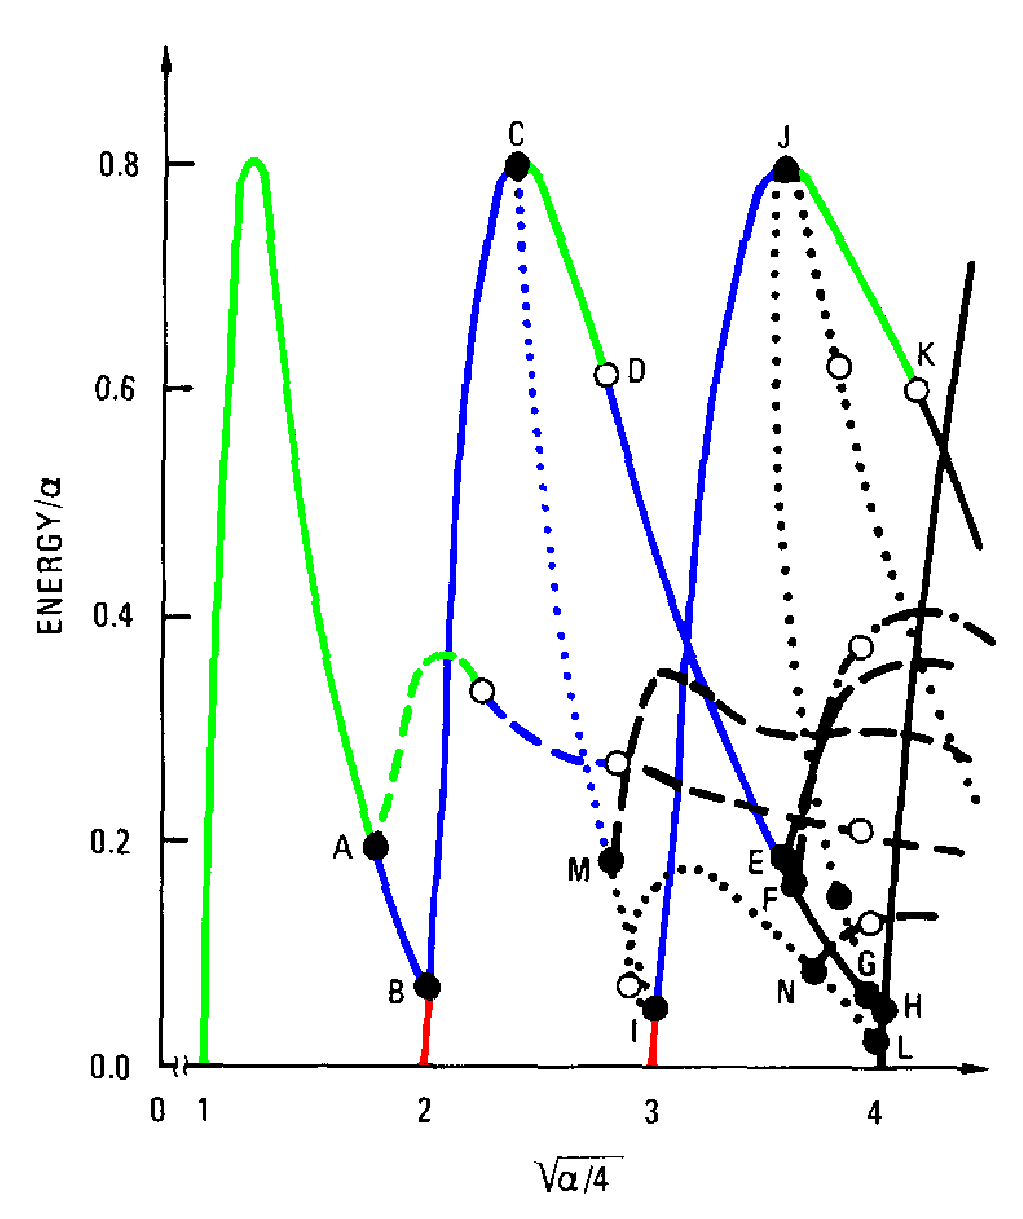
\includegraphics[width=0.5\textwidth]{GreeneKimBifColor}
    % \vspace*{-5pt}
\caption{
    {\small
The ``energy'' of \eqva\ as a function of the bifurcation
parameter $\tildeL=\sqrt{\alpha}/2$, from \refref{ksgreene88}.
The solid curves denote $N$-cell solutions,
dotted curves GLMRT, the dash-dotted curve the
giant states, and dashed curves the propagating solutions.
Open circles indicate Hopf bifurcations.
We have color-coded the branches to reflect the number of unstable
eigenvalues (or complex pairs). Red: 2 unstable eigenvalues, Blue: 1
unstable eigenvalue, Green: stable. Solutions not
resolved in \refref{ksgreene88} or of no interest
to our present purposes have been left black.
        } %end \small
        }
\label{fig:GreeneKim}
    % \vspace*{-5pt}
\end{figure}
%%%%%%%%%%%%%%%%%%%%%%%%%%%%%%%%%%%%%%%%%%%%%%%%%%%%%%%%%%%%%%%%%%

Greene and Kim study extends the earlier work\rf{Mks86,laquey74}
on the \KS\ \eqva\ and their bifurcations. The
bifurcation diagram \reffig{fig:GreeneKim} summarizes the results
relevant to the system sizes studied here.
\PC{
Please redraw bifurcation diagram \reffig{fig:GreeneKim} from the
scratch in xfig (that will make it easier for me to edit), labeling
the axes with our symbols, and various \eqva\ with our - still in flux -
notation for them. Indicate also by circles the nature of
bifurcations for $u(x) = 0$ \eqv. I though those were Hopf? Wrong?
For the thesis, make schematic plots of each bifurcation,
in style of Strogatz or whatever standard textbook on bifurcations
you like the best. You will help Jonathan and me understand what precisely
these bifurcations are. Thanks!
    }
\PC{indicate Christiansen at al. and Lan and Cvitanovi\'c  choices of
    system size on the $\tildeL$ axis
    in \reffig{fig:GreeneKim}. Might require thinking - they are
    in the antisymmetric subspace, I tend to 1/2 them but here one should
    not.}

For small $\alpha$ the only \eqv\ of the system is the constant solution $y(x,t)=0$,
which is globally attracting
for $\tildeL=\sqrt{\alpha}/2<1$. At $\tildeL=N$, with $N$ integer,
the $N$th harmonic becomes unstable and the constant solution
bifurcates to the so called $N$-cell states.
These states contain only the multiples of the $N$th
harmonic, {\ie} only the components $a_N,a_{2N},...$ in our notation.
Moreover, the $N$-cell states are found to be symmetric (in our case, since $u=y_x$ they will be
antisymmetric).
Greene and Kim show that symmetric solutions are \eqva, not \reqva.
At point $A$ in \reffig{fig:GreeneKim} the $1$-cell state loses stability
and bifurcates to a stable,
asymmetric \reqv, which later on becomes unstable through a Hopf bifurcation.
\PC{harmonize our notation with the ``$N$-cell state" notation}

At $\tildeL=2$ the system has become large enough that a $2$-cell \eqv\ appears. At point $B$
in \reffig{fig:GreeneKim} the $1$-cell branch merges to the $2$-cell branch. In general each $N$-cell branch merges to the corresponding $2N$-cell branch.

At point $C$ in \reffig{fig:GreeneKim} the $2$-cell state bifurcates to a type of
\eqv\ solution
found by La Quey, Mahajan, Rutherford and Tang\rf{laquey74} and generalized by Greene and Kim who refer to them as GLMRT \eqva. GLMRT solutions are symmetric
($u(x)$ is antisymmetric)
and can be roughly described as long-wave distorted $N$-cell states.

The last type of solution identified in \refref{ksgreene88} appears at point $F$
in \reffig{fig:GreeneKim} and is called a
``giant" state because its amplitude grows as the system size increases.

According to the bifurcation diagram \reffig{fig:GreeneKim},
at the point that corresponds to system size $\tildeL=\alpha^{1/2}/2=3.501$
studied here,
the {\eqva} we expect are the $2$- and $3$-cell states ($\EQV{2}$ and $\EQV{3}$ respectivelly), the GLMRT state that bifurcates from a $3$-cell state at point $I$ ($\EQV{1}$),
the \reqva\ that belong to the branches starting at points $A$ ($\REQV{\pm}{1}$),
and $M$ ($\REQV(\pm){2}$).

%%%%%%%%%%%%%%%%%%%%%%%%%%%%%%%%%%%%%%%%%%%%%%%%%%%%%%%%%%%%%%%%
\begin{figure}[t]
    % \vspace*{-5pt}
\centering
%RESTORE? 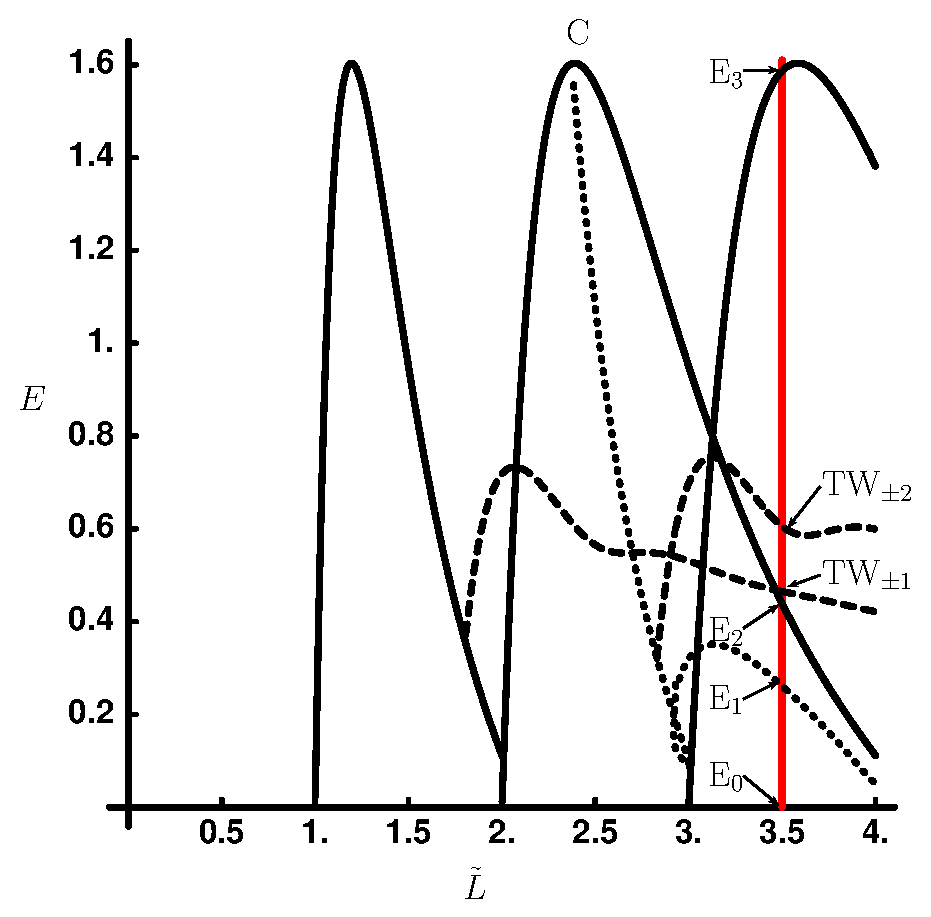
\includegraphics[width=0.5\textwidth]{ksBifDiag}
    % \vspace*{-5pt}
\caption{
    {\small
    Preliminary version of bifurcation diagram for equilibria of \KSe.  Shown is the 2c to GLMRT bifurcation and the GLMRT to $\REQV{\pm}{2}$ bifurcation, points C and M in \rf{ksgreene88} respectively. The traveling wave branch is followed up to our system size.} %end \small
        }
\label{fig:ksBifDiag}
    % \vspace*{-5pt}
\end{figure}
%%%%%%%%%%%%%%%%%%%%%%%%%%%%%%%%%%%%%%%%%%%%%%%%%%%%%%%%%%%%%%%%%%

\subsection{Back in the saddle again}

Kevrekidis, Nicolaenko and Scovel~\rf{KNSks90} study \KSe\ steady state
bifurcations and the role of symmetry in the existance of structurally stable (relative) homoclinic and heteroclinic connections between unstable saddles. The form  of the equation they use is
essentially that of Greene and Kim but with bifurcation parameter connected to our by $\alpha=4\tilde{L}^2$.


They prove that the bifurcation of the trivial state $y=0$ to an $N$-cell state is a pitchfork.
They observe that when the $1$-cell state losses stability at point $A$ the
eigenvector corresponding to the zero eigenvalue of the stability matrix aligns itself with the direction of uniform translation of the
system which, due to the translational invariance of \KSe\, also corresponds to a zero eigenvalue. Thus the algebraic multiplicity of the zero eigenvalue is $2$ while its geometric multiplicity is $1$. Using this fact and a local, $O(2)$-equivariant, approximation to the center manifold they prove that this type of bifurcation creates traveling waves.

In typical numerical simulations  a trajectory initiated along the (single) unstable eigendirection of a
fixed point $y$ of the $2$-cell branch would eventually become attracted to the $L/4$-translated equilibrium $y'$.
Those (relative) homoclinic connections
\ES{In \refref{KNSks90} the characterization homoclinic connection is used. Here
we prefer (to invent?) the term relative homoclinic to emphasize the fact that the fixed points are symmetry related.} although structurally unstable in most dynamical systems, were found to be persistent in KSe with the afore-mentioned behaviour observed in the range
from $\tilde{L}\simeq 2.009$ up to $\tilde{L}\simeq 2.375$  where the $2$-cell state becomes stable. The existance and
robustness of the saddle connection was explained as follows\ES{The following may not make perfect sense without reading the paper, especially the
notation. I've start re-writing \KS\ symmetries section to incorporate information about the invariant subspaces which hopefully will explain it but
my progress is very slow.}:  The unstable manifold of $y$ lies on an invariant subspace $L$ of
\KS\ flow, which is the fixed set of the isotropy subgroup of $O(2)$ defined by reflection with respect to imaginary axis. The action of the generator of $D(4)$ (which sents y to y') on $L$ is to send it to the invariant subspace $R_{1}$ which is the fixed set of $Z(2)$ defined by complex
conjugation. The converse is also true, i.e. the action of $D(4)$ sents $R_{1}$ to $L$. Thus the unstable eigendirection of $y$, lying on $L$, is sent on $R_{1}$ for the $L/4$-shifted point $y'$. The two invariant subspaces $L$ and $R_{1}$ are orthogonal and thus the point $y'$ has only stable eigendirections on $L$ and appears as a sink on that subspace. This explains why the (relative) homoclinic connections are structurally stable in \KSe.

In the range $\tilde{L}=2.00$ when the $2$-cell branch comes to existance with two unstable eigendirections, up to $\tilde{L} \simeq 2.009$ when it
merges to the $1$-cell branch and losses one of its unstable eigendirections, a heteroclinic loop exists that connects $2$-cell to $1$-cell solutions.
The analysis is similar to the previous case.

An important remark in \refref{KNSks90} is that the exact saddle connections were observed using a numerical integrator based on an explicit Galerkin spectral discretezation of \KSe, irrespective of how close to the equilibrium along the unstable manifold we start. On the contrary, when an FFT-based integrator was used, trajectories with initial condition along the unstable direction of $y$ would approach the homoclinic connection but fly away along the direction of the unstable manifold of $y'$ and follow an approximate (relative) homoclinic loop. This is attributed to the Galerkin truncation respecting the symmetries and possesing the same subspaces as the original equation restricted to the first $n$ modes \ES{We observe the second kind of behavour and we both use an FFT based integrator. I plan to quikly write a Galerkin integrator and check to see if we get an exact connection.}.
